\chapter{MISCELLANEOUS \label{cha:appendix}}

\TAMUTocAddWordPage

\section{Figures/Tables in Appendix}

\begin{figure}[!htbp]
\begin{center}
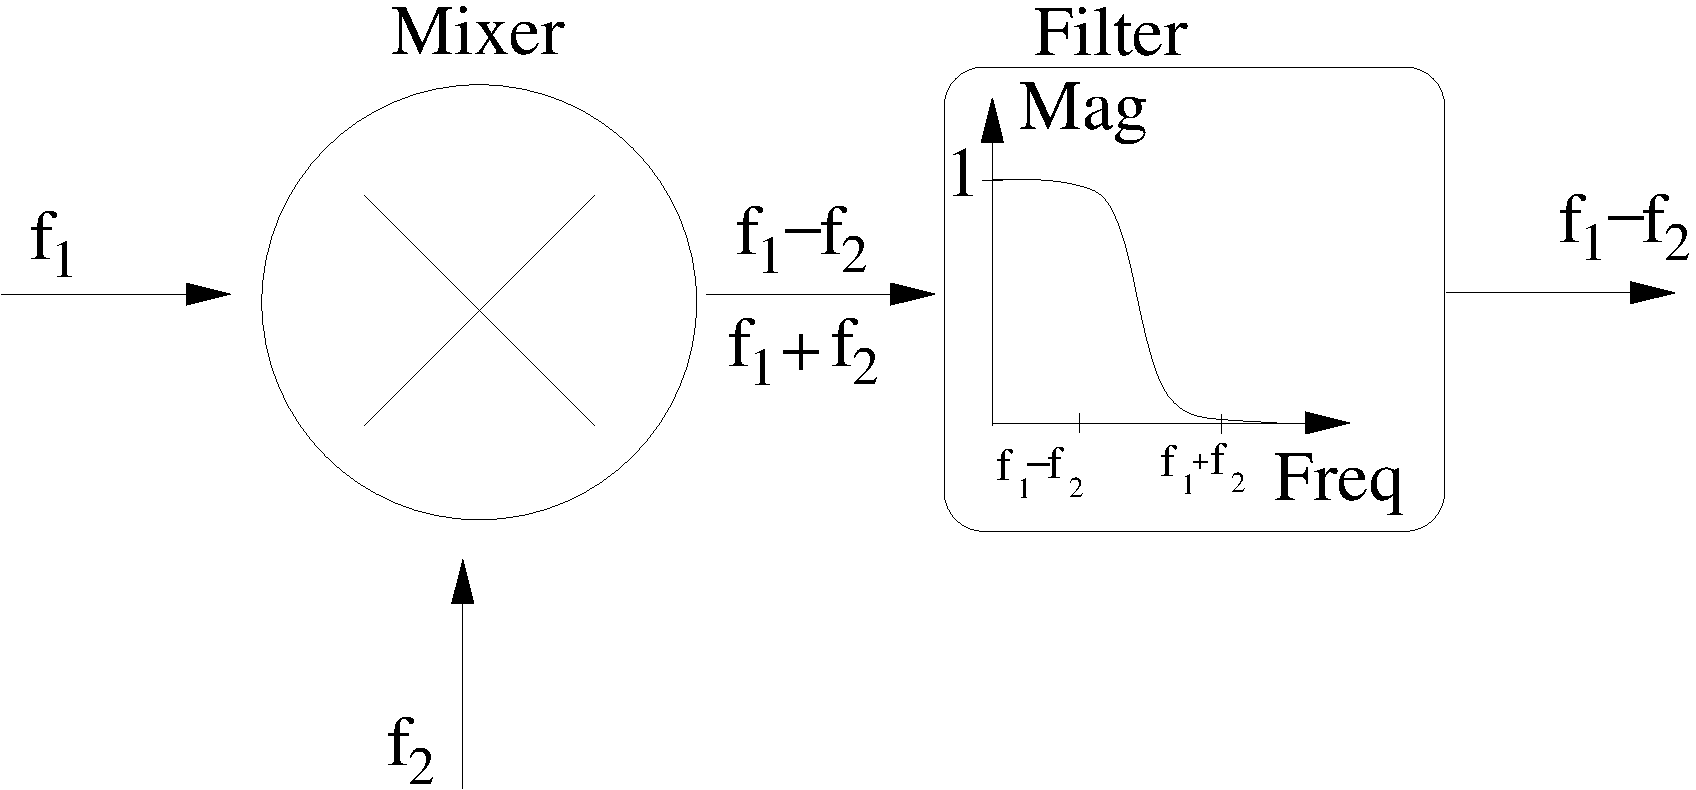
\includegraphics[width=\textwidth]{graphic/analogue_mixer.pdf}
\caption{Test Picture for lof (List of Figures) Display Test Purpose Only}
[The file used is in PDF format.]
\label{fig:chirpHardware}
\end{center}
\end{figure}


\begin{figure}[!htbp]
\begin{center}
\includegraphics[width=\textwidth]{graphic/TestPattern1.bmp}
\caption{CS4270 Test Bench 1 FPGA Design Diagram}
\label{fig:cs4270test1}
{\small [Picture is for test display purpose only. No meaning.]}
\end{center}
\end{figure}

\subsection{TEST1}
Test subsection for toc display purpose only.

\begin{figure}[!hbp]
\begin{center}
\includegraphics[width=\textwidth]{graphic/TESTOUT3_2bit_2.bmp}
\caption{Behavioral simulation for \textbf{TEST1}}
\label{fig:behaviorSimTest1}
{\small [Picture is for test display purpose only. No meaning.]}
\end{center}
\end{figure}


\subsection{TEST2}
\begin{verbatim}
		begin
			if (shift == 1'b1)
			begin
				sr[(N-1):1] <= sr[(N-2):0];
				sr[0] <= sr_in;				
			end
			else
			begin
				sr[(N-1):1] <= sr[(N-2):0];
				sr[0] <= sr[(N-1)];
			end
		end
\end{verbatim}

\section{Random Pictures and Test}
Section here is to test toc display purpose only.
\section{Misc Test}
Section here is to test toc display purpose only.


\chapter{SOURCE CODE \label{cha:appendixB}}

There is certain trick to display the third page word `Page` in the toc. The code from package {afterpage} below needs to specifically used at certain places. Please read the source code in this Appendix.tex file to locate the position of the code below.
 
\begin{verbatim}
	\TAMUTocAddWordPage
\end{verbatim}

\section{Misc Test 2}
Section here is to test toc display purpose only.
\section{Misc Test 3}
Section here is to test toc display purpose only.

\section{Resource Usage \label{cha:appendixC}}
\begin{landscape}
\begin{verbatim}
Design Summary (This page shows how to use landscape format in Appendix.)
--------------
Design Summary:
Number of errors:      0
Number of warnings:    0
Logic Utilization:
  Number of Slice Flip Flops:         3,899 out of  33,280   11%
  Number of 4 input LUTs:             3,717 out of  33,280   11%
Logic Distribution:
  Number of occupied Slices:          2,198 out of  16,640   13%
    Number of Slices containing only related logic:   2,198 out of   2,198 100%
    Number of Slices containing unrelated logic:          0 out of   2,198   0%
      *See NOTES below for an explanation of the effects of unrelated logic.
  Total Number of 4 input LUTs:       3,890 out of  33,280   11%
\end{verbatim}
\end{landscape}

% Table generated by Excel2LaTeX from sheet 'Sheet4'
\begin{landscape}
%\begin{sidewaystable}[!hbtp]

\begin{table}[!hbtp]
  \begin{center}
% Table generated by Excel2LaTeX from sheet 'Sheet1'
  \caption{Summary of Equipment Used}
  \label{tab:equpiment}%

    \begin{tabular}{|l|l|l|}
    \hline
% \toprule
%    \multicolumn{3}{c}{Equipment For Testing \& Measurement}  \\	\hline
    %\midrule
    \textbf{NAME} 				& 	\textbf{NO.} 	& 	\textbf{COMMENT} \\	\hline
    Tektronix TDS7704B Scope 		& 	1     			& 	7GHz, 20GSa/s time-equivallent sampling oscilloscope \\	\hline
    Tektronix P7240 Probe 			& 	2     			& 	4GHz Single Ended Active Probe(High Impedance) \\	\hline
    Agilent 81130A Function Generator 	& 	1     			& 	2 CHs Signal Generator \\	\hline
    Xilinx Spartan-3A DSP 1800A Demo Board & 1     			& 	http://goo.gl/Svvpy \\	\hline
%    \bottomrule
    \end{tabular}%
    
        [{\small By University Requirement, no text should be allowed here in this landscape table/picture page. \textbf{ DON''T USE sidewaystable from rotating package, it cannot align landscape title to the left binding side.}}]
        \end{center}
\end{table}

\end{landscape}

